\documentclass[tikz,border=5mm]{standalone}
\usepackage{pgfplots}
\usepackage{amsmath}
\pgfplotsset{compat=1.18}

\definecolor{planeblue}{RGB}{120, 195, 220}
\definecolor{triedge}{RGB}{0, 60, 220}
\definecolor{linepurple}{RGB}{128, 0, 128}
\definecolor{interred}{RGB}{204, 24, 66}

\begin{document}
	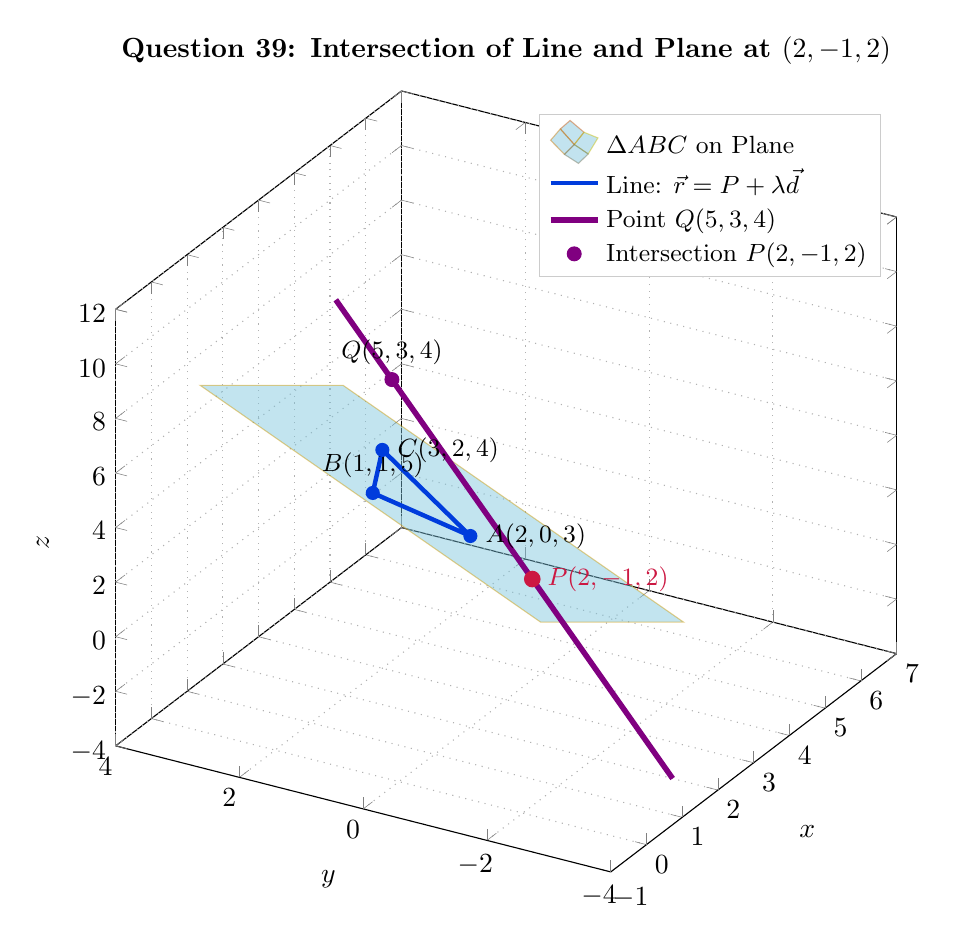
\begin{tikzpicture}
		\begin{axis}[
			width=11.5cm, height=11.5cm,
			view={-60}{30},
			title={\textbf{Question 39: Intersection of Line and Plane at $(2, -1, 2)$}},
			xlabel={$x$}, ylabel={$y$}, zlabel={$z$},
			xmin=-1, xmax=7,
			ymin=-4, ymax=4,
			zmin=-4, zmax=12,
			xtick={-1, 0, 1, 2, 3, 4, 5, 6, 7},
			ytick={-4, -2, 0, 2, 4},
			ztick={-4, -2, 0, 2, 4, 6, 8, 10, 12},
			grid=both,
			grid style={dotted, gray!60},
			legend cell align={left},
			legend style={at={(0.98,0.97)}, anchor=north east, font=\small, draw=gray!40}
			]
			% Plane surface x - y + z = 5  =>  z = 5 - x + y
			\addplot3[
			surf, opacity=0.45, fill=planeblue, draw=none,
			domain=0.5:4.5, domain y=-2.0:3.5, samples=2
			] {5 - x + y};
			
			% Triangle ABC on Plane
			\addplot3[triedge, line width=1.6pt] coordinates {
				(2, 0, 3) (1, 1, 5) (3, 2, 4) (2, 0, 3)
			};
			\addlegendentry{$\Delta ABC$ on Plane}
			
			% Line through P(2, -1, 2) and Q(5, 3, 4) -> direction (3, 4, 2)
			\addplot3[linepurple, line width=2pt] coordinates {(-1, -5, 0) (6.2, 4.6, 4.8)};
			\addlegendentry{Line: $\vec{r} = P + \lambda \vec{d}$}
			
			% Point Q(5, 3, 4)
			\addplot3[only marks, mark=*, mark size=2.5pt, linepurple] coordinates {(5, 3, 4)};
			\addlegendentry{Point $Q(5, 3, 4)$}
			
			% Intersection Point P(2, -1, 2)
			\addplot3[only marks, mark=*, mark size=2.8pt, interred] coordinates {(2, -1, 2)};
			\addlegendentry{Intersection $P(2, -1, 2)$}
			
			% Point labels
			\node[circle, fill=triedge, inner sep=1.8pt] at (axis cs:2, 0, 3) {};
			\node[right=2pt, font=\small\bfseries] at (axis cs:2, 0, 3) {$A(2, 0, 3)$};
			
			\node[circle, fill=triedge, inner sep=1.8pt] at (axis cs:1, 1, 5) {};
			\node[above=2pt, font=\small\bfseries] at (axis cs:1, 1, 5) {$B(1, 1, 5)$};
			
			\node[circle, fill=triedge, inner sep=1.8pt] at (axis cs:3, 2, 4) {};
			\node[right=2pt, font=\small\bfseries] at (axis cs:3, 2, 4) {$C(3, 2, 4)$};
			
			\node[above=2pt, font=\small\bfseries, text=black] at (axis cs:5, 3, 4) {$Q(5, 3, 4)$};
			\node[right=2pt, font=\small\bfseries, text=interred] at (axis cs:2, -1, 2) {$P(2, -1, 2)$};
		\end{axis}
	\end{tikzpicture}
\end{document}